\chapter{Results} \label{results}
%% TODO how is correct decided and error defined?
%The results are presented in three sections.
%In section \ref{results:detection} the results of the detection algorithm is presented.
%In section \ref{results:measuring} the results of the measuring algorithm is presented.
%And in section \ref{results:measuring} the overall performance of the system is presented,
%together with the results of online testing.
%
%The results in each category are grouped by: package, distance, height, horizontal position, overall performance. % horizontal position?

\section{Detection} \label{results:detection}
The output of the detection algorithm was compared against ground truth locations of the reference object and package corners, as explained in \ref{benchmarking}.
A detection result was considered to be correct if the error was less than $10\%$, where the error was defined as the sum of distances between the detected points and actual points, divided by the length of the package contour. Table \ref{table:detection_overall} shows the success rates and average error of the detection algorithm.

\begin{table}%[H]
\centering
\begin{tabular}{@{} l *3c @{}}
\toprule
 & {Reference Object}  & {Package}  & {Reference Object and Package}  \\ 
\midrule
Success rate & 0.72 & 0.66 & 0.60 \\ 
Average error & 0.04 & 0.02 & \\
\bottomrule
 \end{tabular}
 \caption{Success rate and average error of detection.}
\label{table:detection_overall}
\end{table}

Table \ref{table:detection_categories} shows the success rates of detection grouped by four categories: package, horizontal angle, distance, and height. Table \ref{table:detection_categories_error} shows the average error grouped in the same way.

\begin{table}[H]
\centering
\begin{tabular}{lcccc}
\toprule
\multicolumn{2}{c}{Category} & Reference Object & Package & Both\\
\midrule

\multirow{5}{*}{Package} 
& 1 & 0.73 & 0.49 & 0.47 \\ 
& 2 & 0.73 & 0.64 & 0.62 \\
& 3 & 0.78 & 0.93 & 0.76 \\
& 4 & 0.62 & 0.53 & 0.49 \\
& 5 & 0.71 & 0.69 & 0.67 \\
\midrule

\multirow{5}{1.5cm}{Horizontal angle}
& Long side		& 0.56 & 0.53 & 0.38 \\ 
& Angle long		& 0.73 & 0.78 & 0.69 \\
& Wide angle 		& 0.91 & 0.87 & 0.87 \\
& Angle short 	& 0.76 & 0.69 & 0.67 \\
& Short side		& 0.62 & 0.42 & 0.40 \\
\midrule
\multirow{3}{*}{Distance ($m$)} 
& 1 			& 0.56 & 0.53 & 0.38 \\ 
& 1.5  			& 0.73 & 0.78 & 0.69 \\
& 2 			& 0.91 & 0.87 &0.87 \\
\midrule
\multirow{3}{*}{Height} 
& Low 		& 0.51 & 0.44 & 0.37 \\ 
& Medium 	& 0.80 & 0.75 & 0.72 \\
& High		& 0.84 & 0.79 & 0.71 \\
\bottomrule
 \end{tabular}
 \caption{Success rate of detection by grouped by different categories.}
\label{table:detection_categories}
\end{table}


\begin{table}%[H]
\centering
\begin{tabular}{lccc}
\toprule
\multicolumn{2}{l}{Category} & Reference Object & Package\\
\midrule

\multirow{5}{*}{Package} 
& 1 & 0.04 & 0.02\\ 
& 2 & 0.04 & 0.03\\
& 3 & 0.04 & 0.03\\
& 4 & 0.04 & 0.01\\
& 5 & 0.04 & 0.03\\
\midrule

\multirow{5}{*}{Rotation}
& Frontal long		& 0.03 & 0.03 \\ 
& Sharp long	& 0.04 & 0.02 \\
& Wide angle 	& 0.04 & 0.02 \\
& Sharp short 	& 0.04 & 0.02 \\
& Frontal short	& 0.04 & 0.03 \\
\midrule
\multirow{3}{*}{Distance ($m$)} 
& 1 			& 0.03 & 0.02  \\ 
& 1.5  			& 0.04 & 0.02  \\
& 2 			& 0.05 & 0.03  \\
\midrule
\multirow{3}{*}{Height} 
& Low 		& 0.04 & 0.02 \\ 
& Medium 	& 0.04 & 0.02 \\
& High		& 0.04 & 0.02 \\
\bottomrule
 \end{tabular}
 \caption{Average relative error of detection by grouped by different categories.}
\label{table:detection_categories_error}
\end{table}


As shown in table \ref{table:detection_by_package} the success rates varied quite much by package, between 0.49 and 0.76 for detection of both the reference object and package in the same image.
\begin{table}
\centering
\begin{tabular}{@{} *4c @{}}
\toprule
 \multicolumn{1}{c}{Package $\#$} & {Reference Object}  & {Package}  & {Reference Object and Package}  \\ 
\midrule
 1 & 0.73 & 0.49 & 0.47 \\ 
 2 & 0.73 & 0.64 & 0.62 \\
 3 & 0.78 & 0.93 & 0.76 \\
 4 & 0.62 & 0.53 & 0.49 \\
 5 & 0.71 & 0.69 & 0.67 \\
\bottomrule
 \end{tabular}
 \caption{Successful detection rates by package.}
\label{table:detection_by_package}
\end{table}

The results varied even more by horizontal position, where the detection rates of reference object and package were between 0.38 and 0.87, as shown in table \ref{table:detection_by_position}.
\begin{table}
\centering
\begin{tabular}{@{} l *3c @{}}
\toprule
 \multicolumn{1}{c}{Position} & Reference Object  & Package  & Reference Object and Package  \\ 
\midrule
 Frontal long side 			& 0.56 & 0.53 & 0.38 \\ 
 Sharp angle by long side  	& 0.73 & 0.78 & 0.69 \\
 Wide angle 				& 0.91 & 0.87 & 0.87 \\
 Sharp angle by short side 	& 0.76 & 0.69 & 0.67 \\
 Frontal short side 		& 0.62 & 0.42 & 0.40 \\
\bottomrule
 \end{tabular}
 \caption{Successful detection rates by position.}
\label{table:detection_by_position}
\end{table}

As shown in table \ref{table:detection_by_distance}, detection rates by distance were about the same for the distances 1 and 1.5 metres at 0.68 and 0.73 respectively, but fell substantially for the distance 2 metres to 0.39.
\begin{table}[H]
\centering
\begin{tabular}{@{} *4c @{}}
\toprule
 \multicolumn{1}{c}{Distance ($m$)} & Reference Object  & Package  & Reference Object and Package  \\ 
\midrule
 1 	& 0.84 & 0.72 & 0.68 \\ 
 1.5 & 0.84 & 0.77 & 0.73 \\
 2 	& 0.47 & 0.48 & 0.39 \\
\bottomrule
 \end{tabular}
 \caption{Detection by distance to the centre of the package.}
\label{table:detection_by_distance}
\end{table}

As shown in table \ref{table:detection_by_height}, detection rates by height were significantly lower for the lowest height, and about the same for the two higher, at 0.72 and 0.71.
\begin{table}[H]
\centering
\begin{tabular}{@{} l *3c @{}}
\toprule
 \multicolumn{1}{c}{Height ($m$)} & Reference Object  & Package  & Reference Object and Package  \\ 
\midrule
 Low 		& 0.51 & 0.44 & 0.37 \\ 
 Medium 	& 0.80 & 0.75 & 0.72 \\
 High		& 0.84 & 0.79 & 0.71 \\
\bottomrule
 \end{tabular}
 \caption{Detection by height above the ground. For package 1-3 the heights were 0.9 , 1.2 and 1.5 metres. For package 4-5 the heights were 1.1, 1.4 and 1.7 metres.} 
\label{table:detection_by_height}
\end{table}

\section{Measuring} \label{results:measuring} 
The results presented in section were obtained by using ground truth locations of the corners as input to the measuring algorithm, and comparing the output against the manually measured dimensions of the packages.
A measurement was considered to be correct if no dimension of the package had a relative error greater than $10\%$.
The error column in the tables below states the sum of relative errors. 
Table \ref{table:measurement_overall} shows that vanishing point calibration have slightly lower success rate than Zhang's method, and marginally larger error.

(TODO split error to xyz components since vp calibration and zhang uses same xy) % TODO dela upp felet i xyz eftersom calib och vp använder samma xy

\begin{table}[H]
\centering
\begin{tabular}{@{} *4c @{}}
\toprule
\multicolumn{2}{c}{Vanishing point calibration} & \multicolumn{2}{c}{Zhang's method}\\ 
\cmidrule(r){1-2}
\cmidrule(r){3-4}
Success rate & Error & Success rate & Error \\
\midrule
 0.81 & 0.08 & 0.93 & 0.07 \\ 
\bottomrule 
 \end{tabular}
 \caption{Measurement overall.}
\label{table:key_measurement_overall}
\end{table}



% TODO text?

\begin{table}
\centering
\begin{tabular}{@{} *5c @{}}
\toprule
\multirow{2}{*}{Package$~\#$} & \multicolumn{2}{c}{Vanishing point calibration} & \multicolumn{2}{c}{Zhang's method}\\ 
\cmidrule(r){2-3}
\cmidrule(r){4-5}
& Success rate & Error & Success rate & Error \\
\midrule
 1 & 0.87 & 0.09 & 0.89 & 0.08 \\ 
 2 & 0.84 & 0.07 & 0.98 & 0.06 \\
 3 & 0.84 & 0.07 & 0.96 & 0.06 \\
 4 & 0.71 & 0.10 & 0.89 & 0.09 \\
 5 & 0.80 & 0.07 & 0.96 & 0.06 \\
\bottomrule 
 \end{tabular}
 \caption{Successful measurement rates by package.}
\label{table:key_measurement_by_package}
\end{table}



Table \ref{table:key_measurement_by_position} shows that the two horizontal positions ($\leftarrow$ what's a better word for this? TODO) from which only two positions can be seen have a significantly lower success rate than the other positions, especially for vanishing point calibration. % TODO comment: what's a better word for this? TODO 

\begin{table}[H]
\centering
\begin{tabular}{@{} l *4c @{}}
\toprule
\multirow{2}{*}{Position} & \multicolumn{2}{c}{Vanishing point calibration} & \multicolumn{2}{c}{Zhang's method}\\ 
\cmidrule(r){2-3}
\cmidrule(r){4-5}
& Success rate & Error & Success rate & Error \\
\midrule
 Frontal long side 			& 0.56 & 0.07 & 0.84 & 0.07 \\ 
 Sharp angle by long side  	& 0.84 & 0.08 & 0.91 & 0.08 \\
 Wide angle 				& 0.98 & 0.08 & 0.98 & 0.08 \\
 Sharp angle by short side 	& 0.98 & 0.08 & 1.00 & 0.08 \\
 Frontal short side 		& 0.71 & 0.08 & 0.93 & 0.08 \\
\bottomrule
 \end{tabular}
 \caption{Measurement by horizontal position.}
\label{table:key_measurement_by_position}
\end{table}

Table \ref{table:key_measurement_by_distance} show that success rate and accuracy decrease as the distance to the package grows for both methods. Table \ref{table:key_measurement_by_height} shows that the vanishing point method is relatively unaffected by difference in height, while the success rate when using Zhang's calibration method increases as height grows.

\begin{table}
\centering
\begin{tabular}{@{} *5c @{}}
\toprule
\multirow{2}{*}{Distance} & \multicolumn{2}{c}{Vanishing point calibration} & \multicolumn{2}{c}{Zhang's method}\\ 
\cmidrule(r){2-3}
\cmidrule(r){4-5}
& Success rate & Error & Success rate & Error \\
\midrule
 1 		& 0.89 & 0.07 & 1.00 & 0.06 \\ 
 1.5  	& 0.83 & 0.08 & 0.96 & 0.07 \\
 2 		& 0.72 & 0.09 & 0.84 & 0.08 \\
\bottomrule
 \end{tabular}
 \caption{Successful measurement rates by distance.}
\label{table:key_measurement_by_distance}
\end{table}

\begin{table}
\centering
\begin{tabular}{@{} l *4c @{}}
\toprule
\multirow{2}{*}{Distance} & \multicolumn{2}{c}{Vanishing point calibration} & \multicolumn{2}{c}{Zhang's method}\\ 
\cmidrule(r){2-3}
\cmidrule(r){4-5}
& Success rate & Error & Success rate & Error \\
\midrule
 Low 		& 0.80 & 0.08 & 0.87 & 0.07 \\
 Medium 	& 0.83 & 0.08 & 0.95 & 0.07 \\
 High		& 0.81 & 0.08 & 0.99 & 0.08 \\

\bottomrule
 \end{tabular}
 \caption{Successful measurement rates by height above the ground. For package 1, 2 and 3 the heights are $0.9m$, $1.2m$ and $1.5m$. For package 4 and 5 the heights are $1.1m$, $1.4m$ and $1.7m$.} 
\label{table:key_measurement_by_height}
\end{table}

\section{Overall Performance} \label{results:overall}
The results in this section present the performance of the detection and measuring algorithms combined, using vanishing point calibration.
The errors are defined in the same way as in section \ref{results:measuring}.

Table \ref{table:measurement_overall} shows the overall performance of the system , which is $50\%$. However, as can be seen in tables \ref{table:measurement_by_package} - \ref{table:measurement_by_height} some positions are considerably worse than the rest.
These positions are the horizontal positions in which only two sides of the package can be seen, where the distance is 2 metres, and when the height is the lowest (0.9 and 1.1 metres).
If these positions are removed, the results of the remaining, "good positions" give much better results. The success rate for these positions is 0.92, as shown in \ref{table:measurement_overall}.
\\TODO mention the "good positions" in method? % TODO !!!
\\TODO Maybe merge all the small tables to one big table in each section? % TODO !!!
% TODO average result of successful measurements for each package?

\begin{table}[H]
\centering
\begin{tabular}{@{} *4c @{}}
\toprule
\multicolumn{2}{c}{All positions} & \multicolumn{2}{c}{Good positions}\\ 
\cmidrule(r){1-2}
\cmidrule(r){3-4}
Success rate & Error & Success rate & Error \\
\midrule
0.50 & 0.08 & 0.92 & 0.07\\ 
\bottomrule
 \end{tabular}
 \caption{Overall performance for all positions and the optimal positions, respectively.}
\label{table:measurement_overall}
\end{table}


\begin{table}[H]
\centering
\begin{tabular}{@{} *3c @{}}
\toprule
Package$~\#$ & Success rate & Error\\
\midrule
 1 & 0.40 & 0.08 \\ 
 2 & 0.58 & 0.06 \\
 3 & 0.62 & 0.06 \\
 4 & 0.36 & 0.09 \\
 5 & 0.56 & 0.09 \\
\bottomrule 
 \end{tabular}
 \caption{Overall performance by package.}
\label{table:measurement_by_package}
\end{table}



Table \ref{table:measurement_by_position} shows that performance is greatly affected by horizontal position, like earlier. Performance is much worse for the positions from which only two sides of the package can be seen. 

\begin{table}
\centering
\begin{tabular}{@{} l *4c @{}}
\toprule
\multirow{2}{*}{Position} & \multicolumn{2}{c}{Vanishing point calibration} & \multicolumn{2}{c}{Zhang's method}\\ 
\cmidrule(r){2-3}
\cmidrule(r){4-5}
& Success rate & Error & Success rate & Error \\
\midrule
 Frontal long side 			& 0.18 & 0.08 & 0.33 & 0.08 \\ 
 Sharp angle by long side  	& 0.64 & 0.08 & 0.62 & 0.08 \\
 Wide angle 				& 0.80 & 0.06 & 0.82 & 0.06 \\
 Sharp angle by short side 	& 0.62 & 0.08 & 0.62 & 0.07 \\
 Frontal short side 		& 0.27 & 0.10 & 0.33 & 0.10 \\
\bottomrule
 \end{tabular}
 \caption{Successful measurement rates by position.}
\label{table:measurement_by_position}
\end{table}

Bla bla distance table... % TODO

\begin{table}[H]
\centering
\begin{tabular}{@{} *3c @{}}
\toprule
Distance & Success rate & Error\\
\midrule
 1 		& 0.56 & 0.07\\ 
 1.5  	& 0.63 & 0.08\\
 2 		& 0.32 & 0.08\\
\bottomrule
 \end{tabular}
 \caption{Overall performance by distance.}
\label{table:measurement_by_distance}
\end{table}


Bla bla height table... % TODO

\begin{table}[H]
\centering
\begin{tabular}{@{} l *2c @{}}
\toprule
Height & Success rate & Error\\
\midrule
 Low 		& 0.31 & 0.07\\
 Medium 	& 0.65 & 0.07\\
 High		& 0.55 & 0.07\\

\bottomrule
 \end{tabular}
 \caption{Overall performance by height above the ground. For package 1-3 the heights were 0.9 , 1.2 and 1.5 metres. For package 4-5 the heights were 1.1, 1.4 and 1.7 metres.} 
\label{table:measurement_by_height}
\end{table}

\section{Online testing}

Online testing was performed using the Android app described in \ref{method:online_testing}.
A screenshot of the resulting app is shown in figure \ref{fig:screenshot}.
The processing time of the app is typically around 300 milliseconds at the resolution  TODO on the Galaxy S6 Edge, depending on the amount of clutter in the image. % TODO times true?
More clutter results in higher processing times.
% TODO measure time for different resolutions

\begin{figure}[H]
\begin{center}
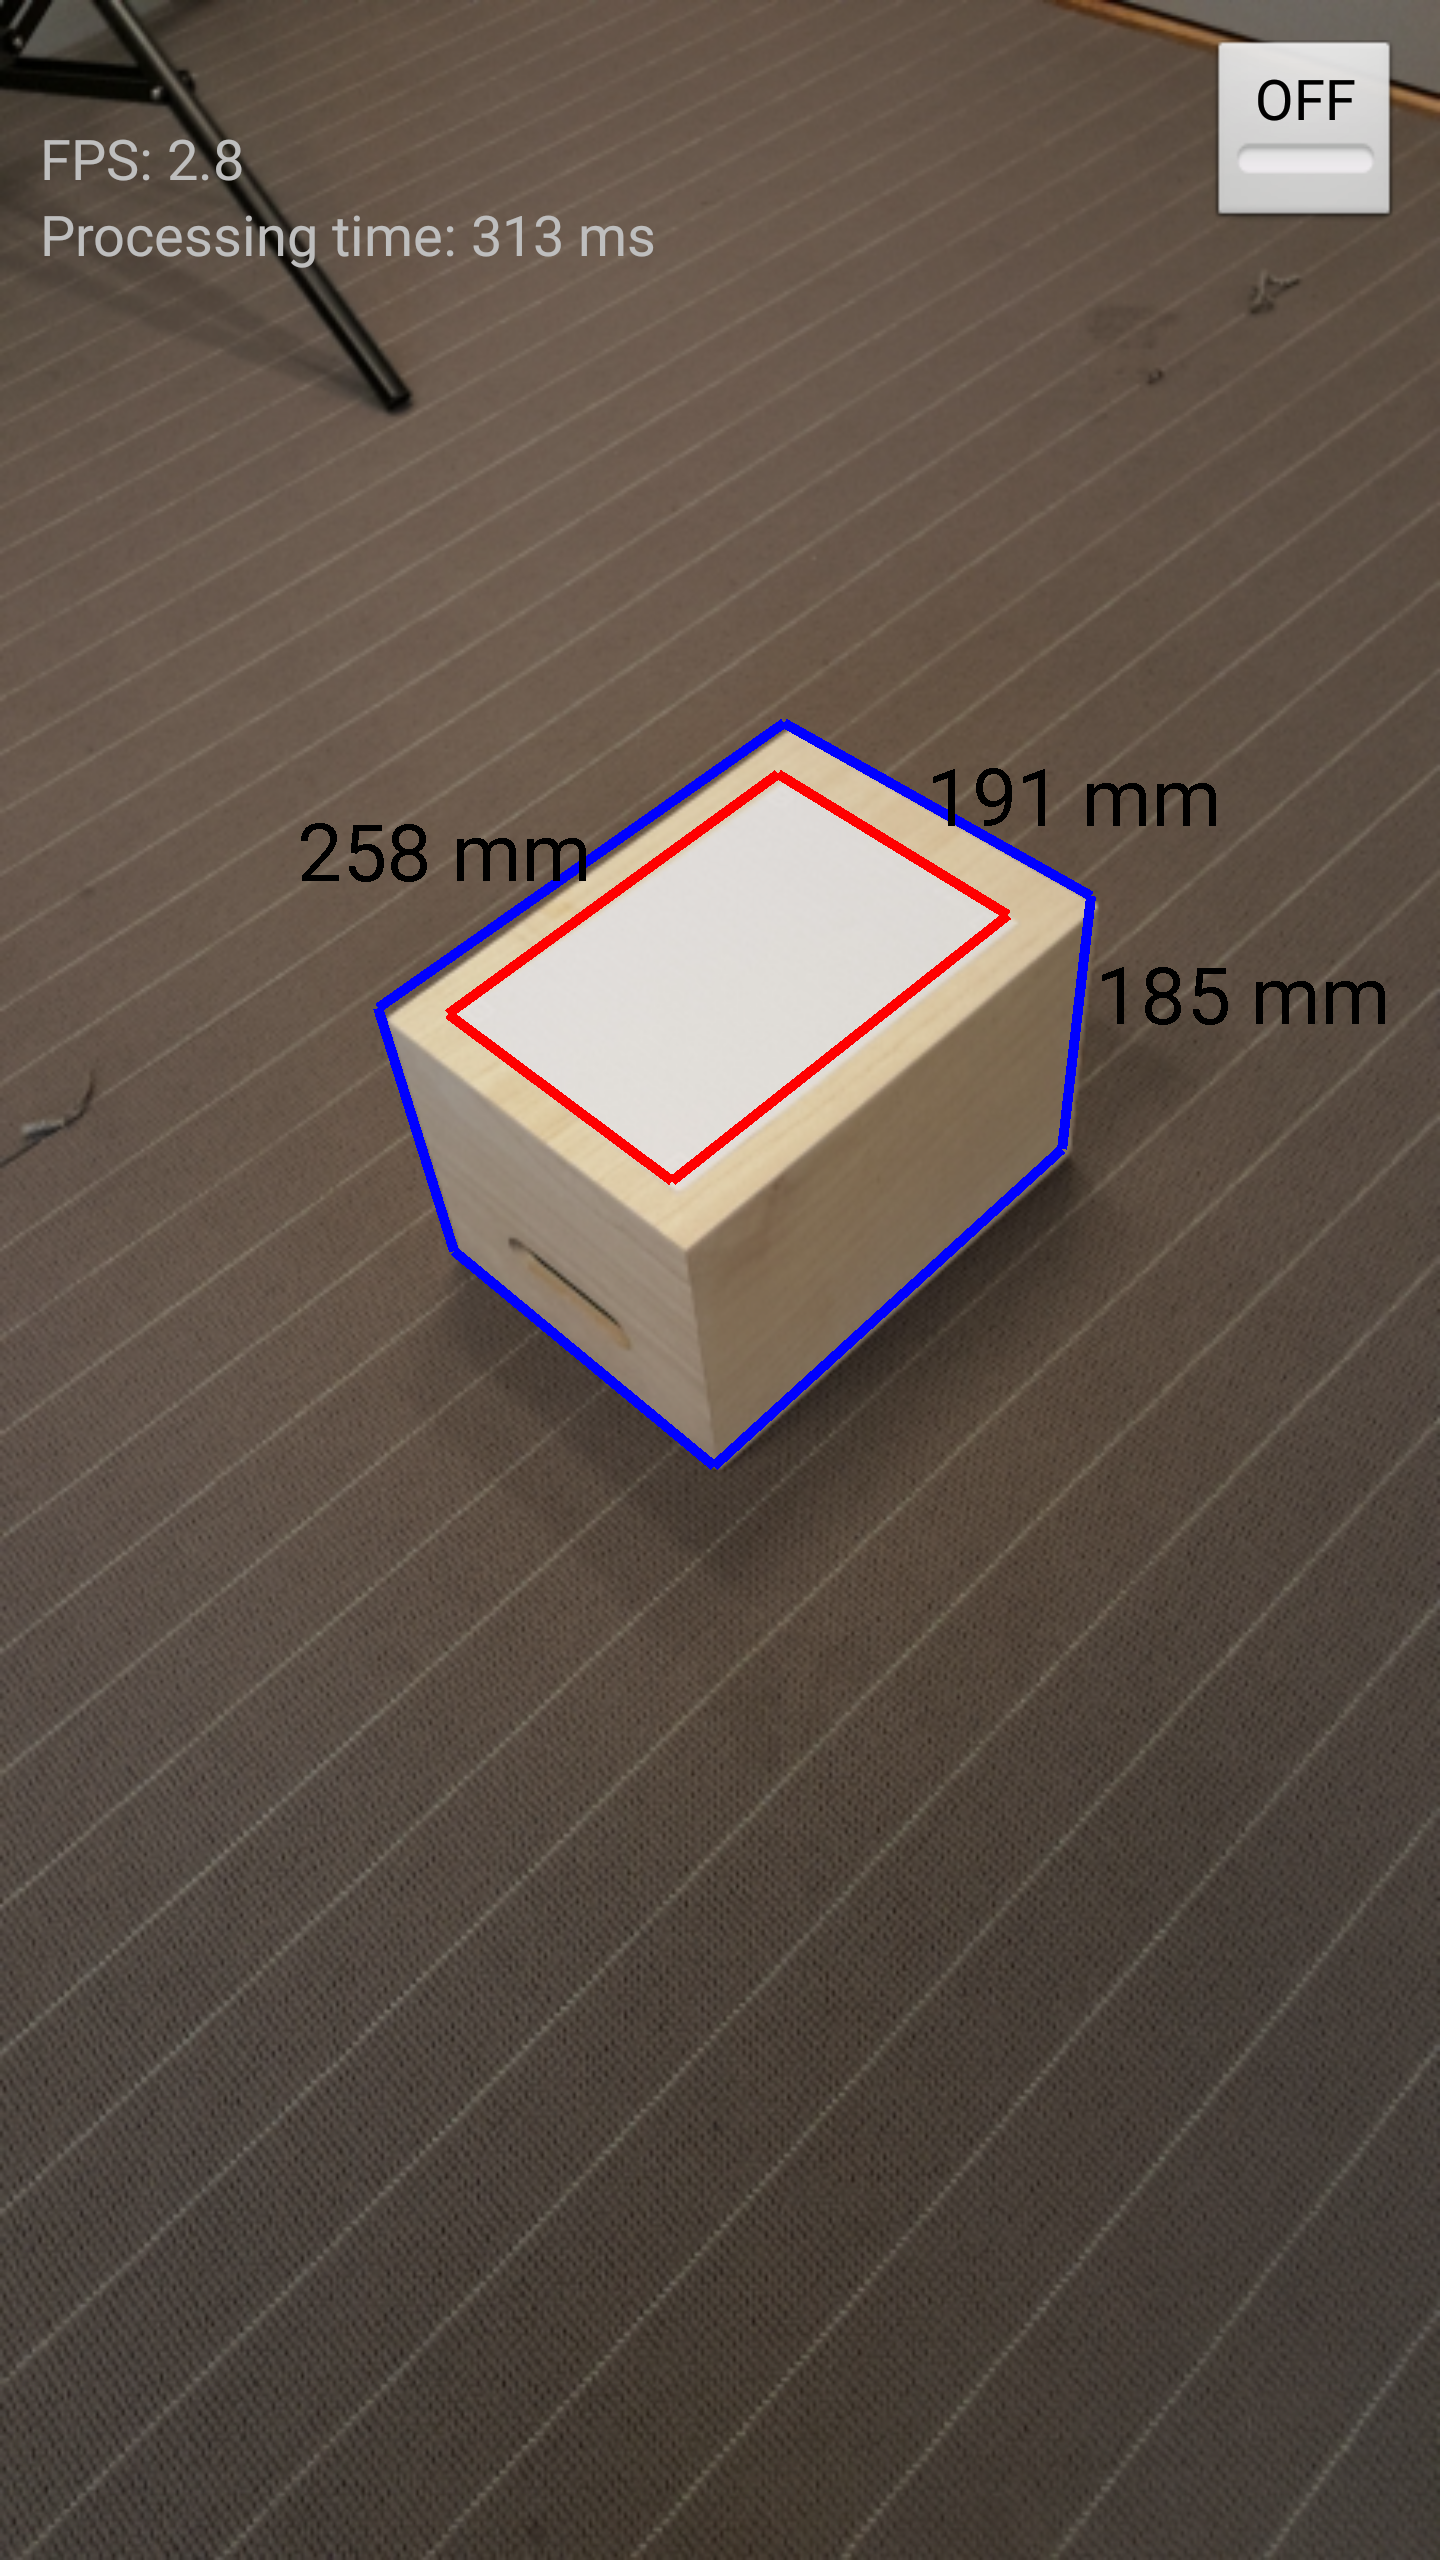
\includegraphics[width=0.6\textwidth]{figures/screenshot.png}
\end{center}
\caption{Screenshot of the app measuring package 2. A blue outline has been drawn around the package, and a red outline has been drawn around the reference object. The real dimensions of the package are $260 \times 191 \times 177$ mm.}
\label{fig:screenshot}
\end{figure}
